\section{Mobile app implementation}
\label{sec:Mobile app implementation}
After the data collection app is implemented, the data collection process begins.
While waiting for the data set to be collected, I designed the deep model as detailed in section \ref{sec:Deep model design}.
After the design of the model is completed, the data loader and the deep model are implemented using Python programming language and TensorFlow framework.
The implementation of EfficientNet (\textit{tf.keras.applications.efficientnet.EfficientNetB0}) and the MLP classification head (\textit{tf.keras.layers.Dense} and \textit{tf.keras.layers.Dropout}) is composed directly from the TensorFlow Keras-style high-level APIs.
The Longformer implementation uses the Hugging Face Transformer\footnote{Hugging Face Transformers: \url{https://huggingface.co/transformers/}} library.
After finish implementing and training the deep model, the remaining research goal is to port the deep model to Android platform.

Although the most widely used programming language for Android development is Java, this project does not use Java except for the automatically generated initialisation codes and native function bindings.
As discussed in section \ref{sec:Framework selection}, the implementation uses React Native to develop UI and application logic.
Even though JavaScript development is more convenient, it is single-threaded and is not suitable for high performance parts in the application.
For the parts that require high performance, such as the image pipeline, the anonymisation process, and the deep model inference process, the C++ programming language is used for multi-threaded Android native development.

\subsection{Architecture overview}
The architecture of the mobile application developed in this research is shown in Figure \ref{fig:4-mobile-arch}.
The arrows in the figure indicate the direction of data flow and clearly show dependencies across different functional blocks.
The left half of the figure describes the user interface and user interaction logic developed using React Native, and the right half describes the core functions of the application developed using C++.
These two parts use React Native Javascript Interface (JSI) for communication.

\begin{figure}[!ht]
    \centering
    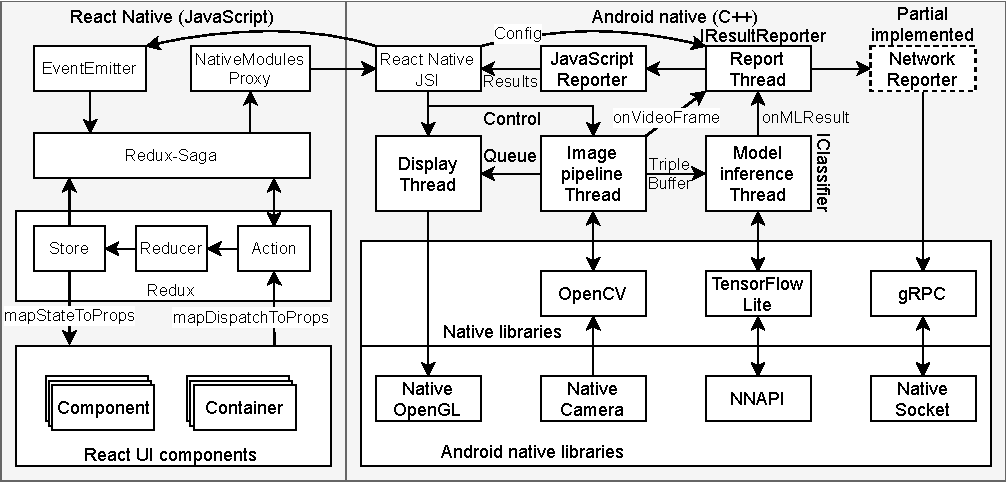
\includegraphics[width=\textwidth]{implementation/imgs/4-mobile-arch.pdf}
    \caption{Mobile app architecture and data flow}
    \label{fig:4-mobile-arch}
\end{figure}

The core functions of this project in the native part shown on the right side in Figure \ref{fig:4-mobile-arch} is much worth discussing than UI implementation on the left side.
These core functions include displaying images without lag and running model inference at the same time.
To achieve the goal, this project implements these functions in C++ by using multi-threading to enable asynchronous processing for display (a real-time task), model inference and network transmission (time-consuming tasks).
It can better take advantage of the multi-core of the mobile phone processor, and time-consuming tasks will not affect the real-time task, which ensures a smooth user experience.

\begin{figure}[!ht]
    \centering
    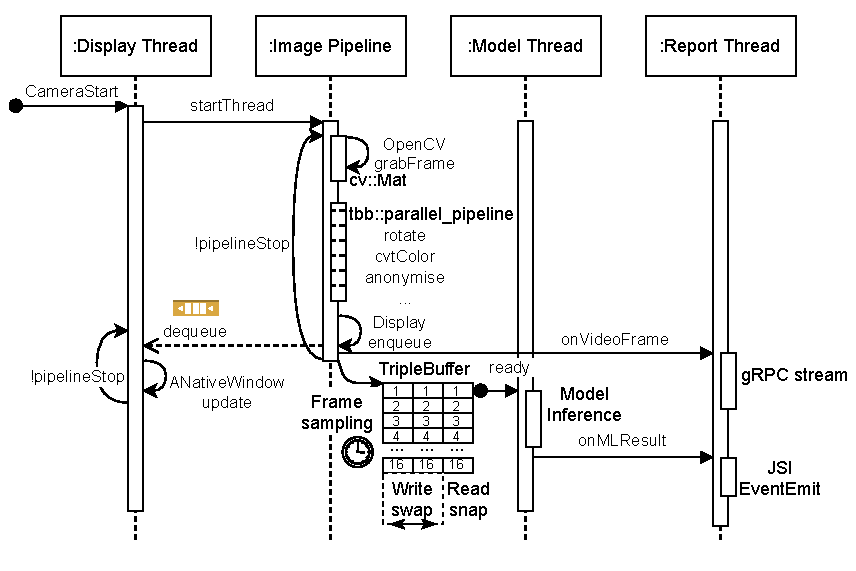
\includegraphics[width=\textwidth]{implementation/imgs/4-model-infer.pdf}
    \caption{Sequence diagram of the multi-threaded app}
    \label{fig:4-model-infer}
\end{figure}
The sequence diagram in Figure \ref{fig:4-model-infer} describes the interactions between four threads in the Android application.
After the user enters the exam screen, the display thread will receive the processed image data through a queue and update the display.
After the exam begins, the model inference thread will be started to receive processed image data from a triple buffer, and performs model inference, then informs the result report thread after getting the result.

The rest of this section will introduce in detail the multi-threaded design for the core function, including display thread, image processing pipeline thread, and model inference thread.

\subsection{Display and image processing pipeline}
This subsection introduces a real-time task involving the display and image processing pipeline in the app.
The image processing pipeline firstly receives an image from a camera on the mobile phone then transforms and anonymises it with OpenCV.
The display thread is responsible for receiving the image processed by the image processing pipeline and showing it through OpenGL.
This process is a real-time task, where the display process takes less time than the image processing process.
The display thread needs to wait for the processed image data from the processing pipeline thread.
Therefore, transferring data across two threads should use the producer-consumer programming paradigm with the blocking queue data structure.

A queue is a commonly used first-in-first-out (FIFO) data structure of a sequential organised collection of entities which can be modified by \textit{enqueue} (adding entities at one end) and \textit{dequeue} (removing entities from the other end).
A thread-safe blocking queue is a queue that may block in \textit{dequeue} operation or \textit{enqueue} operation.
If the blocking queue has already been empty, a \textit{dequeue} operation will block the calling thread until new data are available in the queue.
Conversely, a \textit{enqueue} operation will block the calling thread if the blocking queue has already full.

Algorithm \ref{algo:Image processing pipeline thread} 

\begin{algorithm}[!ht]
\caption{Image processing pipeline thread}
\label{algo:Image processing pipeline thread}

\end{algorithm}

\subsection{Tensorflow Lite adoption and inference}
Although Google provides some ready-made models and easy-to-call Java bindings, it is necessary to use C++ for custom model workflow.
Besides, not all deep models implemented in TensorFlow can be converted to the Lite version due to limited operators compatibility.


As for triple buffering, it is a bridge that connects the image processing thread and model inference thread.
This data structure type has been widely used in the producer-consumer paradigm to deal with the inconsistency of the consumer has a slower speed than the producer.
When the producer is much faster than the consumer, some data loss is inevitable, so it is only necessary to ensure that the consumer gets the latest data in this scenario.

The implementation of triple buffering is an strengthened special case of ring buffering.
In the triple buffering, there are three buffers in the memory, one is snap for reading from the consumer, and the other two are for flip writing from the producer.
When the consumer reads, the newly written buffer will become a reading snap, and then the producer will write the released buffer and the remaining buffer.
Thanks to the atomic operation support provided by C++, \citet{andre2021triple} proposed a lock-free triple buffer implementation for the processes of creating snap and flip writing.

One problem with the initial version of this project is that the model inference thread may read empty data from the triple buffer because the image processing pipeline takes time to produce.
To tinkle this problem, a \textit{readLastBlock} is implemented using mutex and a conditional variable to block the model inference thread until the first set of image data is valid.

\begin{algorithm}[!ht]
\caption{Deep model inference procedure}
\label{algo:Deep model inference procedure}

\end{algorithm}
